% !TEX program = xelatex
% !BIB program = bibtex

\documentclass[UTF8,cs4size]{ctexart}

% layout
\usepackage[left=3cm,right=3cm]{geometry}
\linespread{1.25}
\ctexset{
  section = {
    name = \S
  },
  subsection/name = \S,
  subsubsection/name = \S
}
% \makeatletter
% \def\@seccntformat#1{%
%   \expandafter\ifx\csname c@#1\endcsname\c@section
%   Section \thesection:
%   \else
%   \csname the#1\endcsname\quad
%   \fi}
% \makeatother
 
% page headings
\usepackage{fancyhdr}
\setlength{\headheight}{15.2pt}
\pagestyle{fancy}
\lhead{\leftmark}
\rhead{M201873026 刘一龙}
\cfoot{\thepage}
% \makeatletter
% \let\headauthor\@author
% \makeatother

% url/ref
\usepackage{hyperref}
\hypersetup{
  colorlinks,
  citecolor=black,
  filecolor=black,
  linkcolor=black,
  urlcolor=black,
  pdfauthor={刘一龙},
  pdftitle={人工智能结课报告}
}

% vertical centering title page
\usepackage{titling}
\renewcommand\maketitlehooka{\null\mbox{}\vfill}
\renewcommand\maketitlehookd{\vfill\null}

% table of contents
\usepackage{tocloft}
\renewcommand\cftsecfont{\normalfont}
\renewcommand\cftsecpagefont{\normalfont}
\renewcommand{\cftsecleader}{\cftdotfill{\cftsecdotsep}}
\renewcommand\cftsecdotsep{\cftdot}
\renewcommand\cftsubsecdotsep{\cftdot}
\renewcommand{\contentsname}{\hfill\bfseries\Large 目录\hfill}   
\setlength{\cftbeforesecskip}{10pt}

% figures
\usepackage{graphicx}
\graphicspath{figures/}
% \newcommand\figureht{\dimexpr
%   \textheight-3\baselineskip-\parskip-.2em-
%   \abovecaptionskip-\belowcaptionskip\relax}

% tables
\usepackage{caption} 
\captionsetup[table]{skip=10pt}

% math, algorithms, code
\usepackage{amsmath,amssymb,url}
\usepackage{algorithm, algorithmic}
\usepackage{listings}

\lstset{
   extendedchars=true,
   basicstyle=\footnotesize\ttfamily,
   showstringspaces=false,
   showspaces=false,
   numbers=left,
   numberstyle=\footnotesize,
   numbersep=9pt,
   tabsize=2,
   breaklines=true,
   showtabs=false,
   captionpos=b
}

% bibliography
\usepackage[super,square,comma,sort]{natbib} % for \citet and \citep
\renewcommand{\refname}{\S 参考文献}
% \begin{filecontents}{report.bib}
% \end{filecontents} 

% appendix
\usepackage{appendix}

\title{人工智能结课报告\\ \bigskip \textbf{GBA: 一个基于蒙特卡洛树搜索的简单五子棋人工智能系统}}
\author{计算机科学与技术学院\\ 硕1801\\ M201873026\\ 刘一龙}
\date{\today}

\begin{document}

\pagenumbering{gobble} % no page number
\maketitle
\newpage
\null\thispagestyle{empty}
\newpage

% \pagenumbering{roman}
% \section*{\S 摘要}\sectionmark{\S 摘要}
% \addcontentsline{toc}{section}{\S 摘要}
% \addcontentsline{toc}{section}{\protect\numberline{}\S 摘要}
% \newpage
% \pagenumbering{gobble} % no page number

\tableofcontents
\newpage
\null\thispagestyle{empty}
\newpage

\pagenumbering{arabic}

\section{引言}
游戏 AI 的经典方法要求很高领域知识的质量,或长时间生成有效的AI行为。
这两个特点妨碍建立具有挑战性的游戏AI的目标。
在实现游戏 AI 时,最重要的是评估游戏状态或游戏局势的函数。
经典的方法是使用启发式方法,利用领域知识建立这样的估计函数。
但是,基于启发式方法建立估计函数是一个复杂的任务。
它是复杂游戏环境中游戏 AI 较弱的一个重要原因。

由于 Google DeepMind 的 AlphaGo\cite{DBLP:journals/nature/SilverHMGSDSAPL16}与 AlphaGo Zero\cite{silver2017mastering}的横空出世,
使得人们将目光聚焦至蒙特卡洛树搜索(MCTS,Monte-Carlo Tree Search)\cite{wiki:Monte_Carlo_tree_search}这一上世纪就出现的数学方法。
其又被称为随机抽样或统计试验方法,属于计算数学的一个分支。蒙特卡洛模拟\cite{binder1993monte}最早用于统计物理领域。

其实在很早以前,便有学者提出蒙特卡洛树搜索可以有效地应用于棋盘游戏\cite{DBLP:conf/aiide/ChaslotBSS08}。
蒙特卡罗树搜索作为游戏 AI 的新颖统一框架,通过游戏状态空间的随机探索用来预测最有希望的游戏动作。
最早在 1993 年\cite{brugmann1993monte},就有学者将蒙特卡洛模拟运用在 9x9 的围棋游戏中。
后来有学者将蒙特卡洛树搜索与 UCB(Upper Confidence Bound)相结合提出了 UCT(Upper Confidence Bound Apply to Tree)算法\cite{DBLP:conf/ecml/KocsisS06}。
MoGo 程序\cite{DBLP:conf/cig/WangG07}\cite{DBLP:conf/icml/GellyS07}利用 UCT 算法将自身胜率提升了将近一倍,并成功击败了棋力强劲的围棋业余选手。
10 年后的今天,DeepMind 的学者研制出的 AlphaGo 人工智能更是成功地击败了人类顶尖围棋选手柯洁。

本文提出实现 GBA(GoBang Ai)系统,一个基于蒙特卡洛树搜索的简单五子棋人工智能系统,将最简单的基于 UCT 的蒙特卡洛树搜索策略移植到五子棋游戏上。
本文首先介绍蒙特卡洛搜索树算法,然后阐述 GBA 系统的整体实现,最后阐述该系统中关于对弈算法的关键优化。
\newpage

\section{蒙特卡洛树搜索}
蒙特卡罗树搜索(MCTS),是一种使用随机模拟的最佳优先原则的搜索算法。其基本过程如图~\ref{fig:mcts_phase}所示。
在阶段(1)中,现有信息用于重复选择连续的子节点直到搜索树的末尾。接下来,在阶段(2)中,通过添加节点来扩展搜索树。
然后,在阶段(3)中,模拟运行到最后以确定获胜者。
最后,在阶段(4)中,使用从模拟游戏获得的新信息更新所选路径中的所有节点。
重复运行这种 4 阶段算法,直到收集到足够的信息以产生良好的下一步选择。

\begin{figure}[htb]
  \centering
  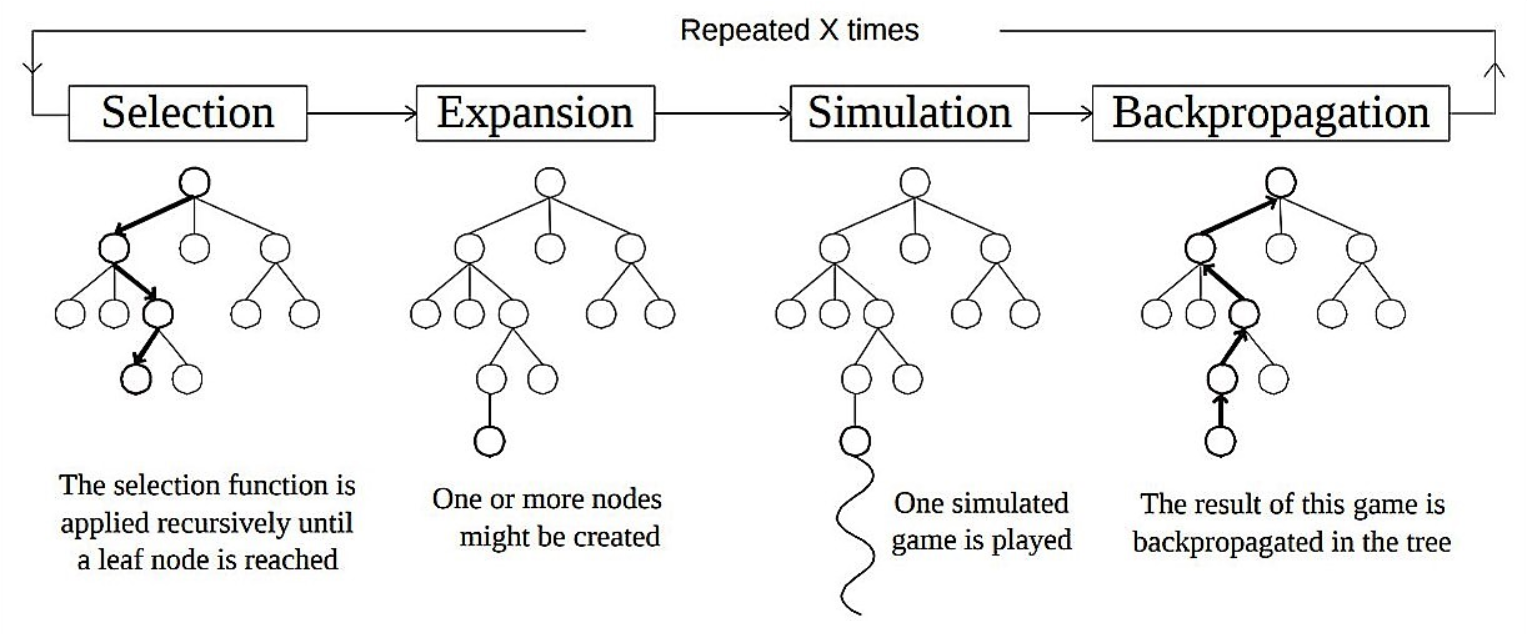
\includegraphics[width=\textwidth,height=5cm]{figures/final_mcts_phase.png}
  \caption{MCTS 算法基本过程\cite{DBLP:conf/aiide/ChaslotBSS08}}
  \label{fig:mcts_phase}
\end{figure}

重要的是要注意搜索树在结构上与游戏树相同,并且搜索树还包含从模拟中收集的统计信息,搜索树是整个游戏树的一个子集。

\subsection{结点选择(Selection)}
在树中找到状态时,根据存储的统计数据选择下一个操作,以便在开发和探索(Exploration Term and Exploitation Term)之间取得平衡。
一方面,任务通常是选择导致迄今为止最佳结果的游戏动作(利用)。 另一方面,由于评估(探索)的不确定性,仍然需要探索不太有希望的行动。
\begin{equation}
  \frac{w_i}{s_i} + c\sqrt{\frac{\ln{s_p}}{s_i}}
  \label{eq:uct}
\end{equation}

\subsection{结点扩展(Expansion)}
\subsection{搜索树模拟(Simulation)}
\subsection{状态回播(Backpropagation)}
\newpage

\section{五子棋系统概述}
\subsection{五子棋游戏框架实现}
\subsection{五子棋人工智能实现}
本文的蒙特卡洛树搜索框架参考了 Michael Liu 的一篇文章\cite{web:medium_mcts}。
\newpage

\section{五子棋对弈算法优化}
\subsection{计分板优化策略}
由于性能限制,如果对于所有空格位置处都进行随机搜索的话,
会使得 GBA 系统在限定的时间内(例如 3 秒) 无法得出最有效的落子选择,
使得其最后的落子选择异常糟糕,造成一种“人工智障”的戏剧场面。

利用计分板策略计算当前棋局局势,得出下一步较为优势的落子集合,缩小搜索树,
可以大幅度提升 GBA 系统的落子选择表现。
\subsection{算法优化结果}
优化前截图

优化后截图
\newpage

\bibliographystyle{unsrt}
\bibliography{bibs/report}
\addcontentsline{toc}{section}{\S 参考文献}
\newpage

\end{document}
